\chapter{Grover's algorithm}

Grover's search algorithm\cite{GroverOriginal} is a quantum algorithm framework, that takes a user-defined solution verifier algorithm (the oracle) and turns it into a $\Theta(\sqrt{N})$ solver. This provides a quadratic speedup over the classical brute force equivalent.

\section{Introduction to Grover's search algorithm framework}

Many sources call this a database search algorithm, since in Grover's original paper it was described as such. However, the 'database' here is an abstract entity, that represents the entire domain of the problem, while the so-called 'marked' elements are the correct solutions in this domain, for which the oracle would return a 'YES' answer. Using the terms 'problem domain' instead of 'database', 'verifier algorithm' insead of 'oracle' and 'solutions' instead of 'marked elements' makes Grover's importance and connection to the P versus NP problem clearer and the details of the algorithm easier to understand.

Another common description of Grover's search algorithm is that it can solve 'unstructured search problems'. What they mean by this is that the algorithm doesn't construct a solution by iterating over partial solutions or improving a non-solution step-by-step. Constrast this with for example how Prim's minimum spanning tree algorithm iterates on partial solutions by connecting the remaining vertices of the graph one at a time. This requires knowledge of the graph and knowledge of how to build a minimal spanning tree one vertex at a time.

Grover doesn't need to know the structure of the original problem, the relationship between partial solutions or how to improve non-solutions. It only needs to know how to verify a solution. It starts by taking all of the entities from the problem's domain with uniform distribution.

\begin{figure}[H]
    \centering
    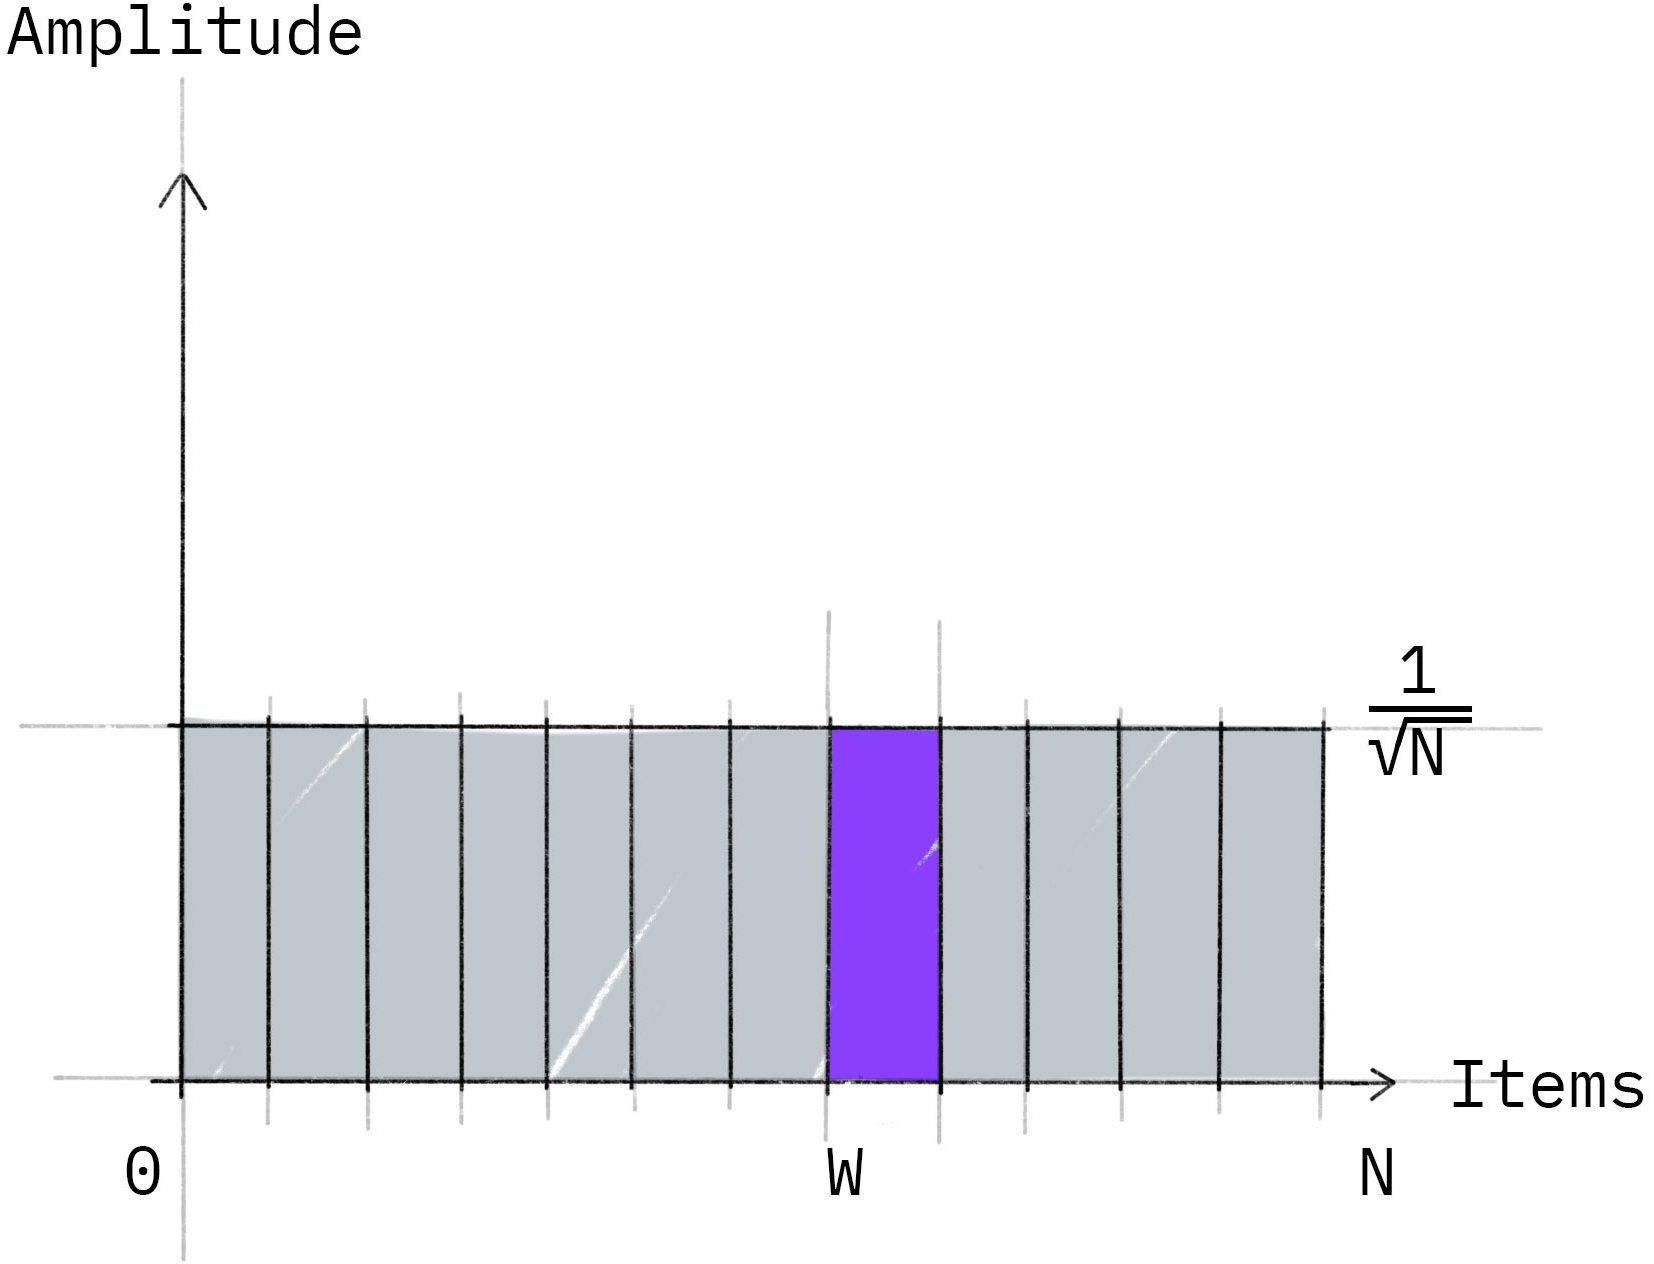
\includegraphics[width=0.5\linewidth]{content/assets/03_grovers_algorithm/grover_uniform.jpg}
    \caption{Grover starts out with the uniform distribution}
    \label{fig:grover_uniform}
\end{figure}

Then, it uses the verifier algorithm in a process to manipulate their probabilities until the correct entities' probabilities are very high, while the incorrect entities' probabilities are very low. This process is called amplitude amplification.

\begin{figure}[H]
    \centering
    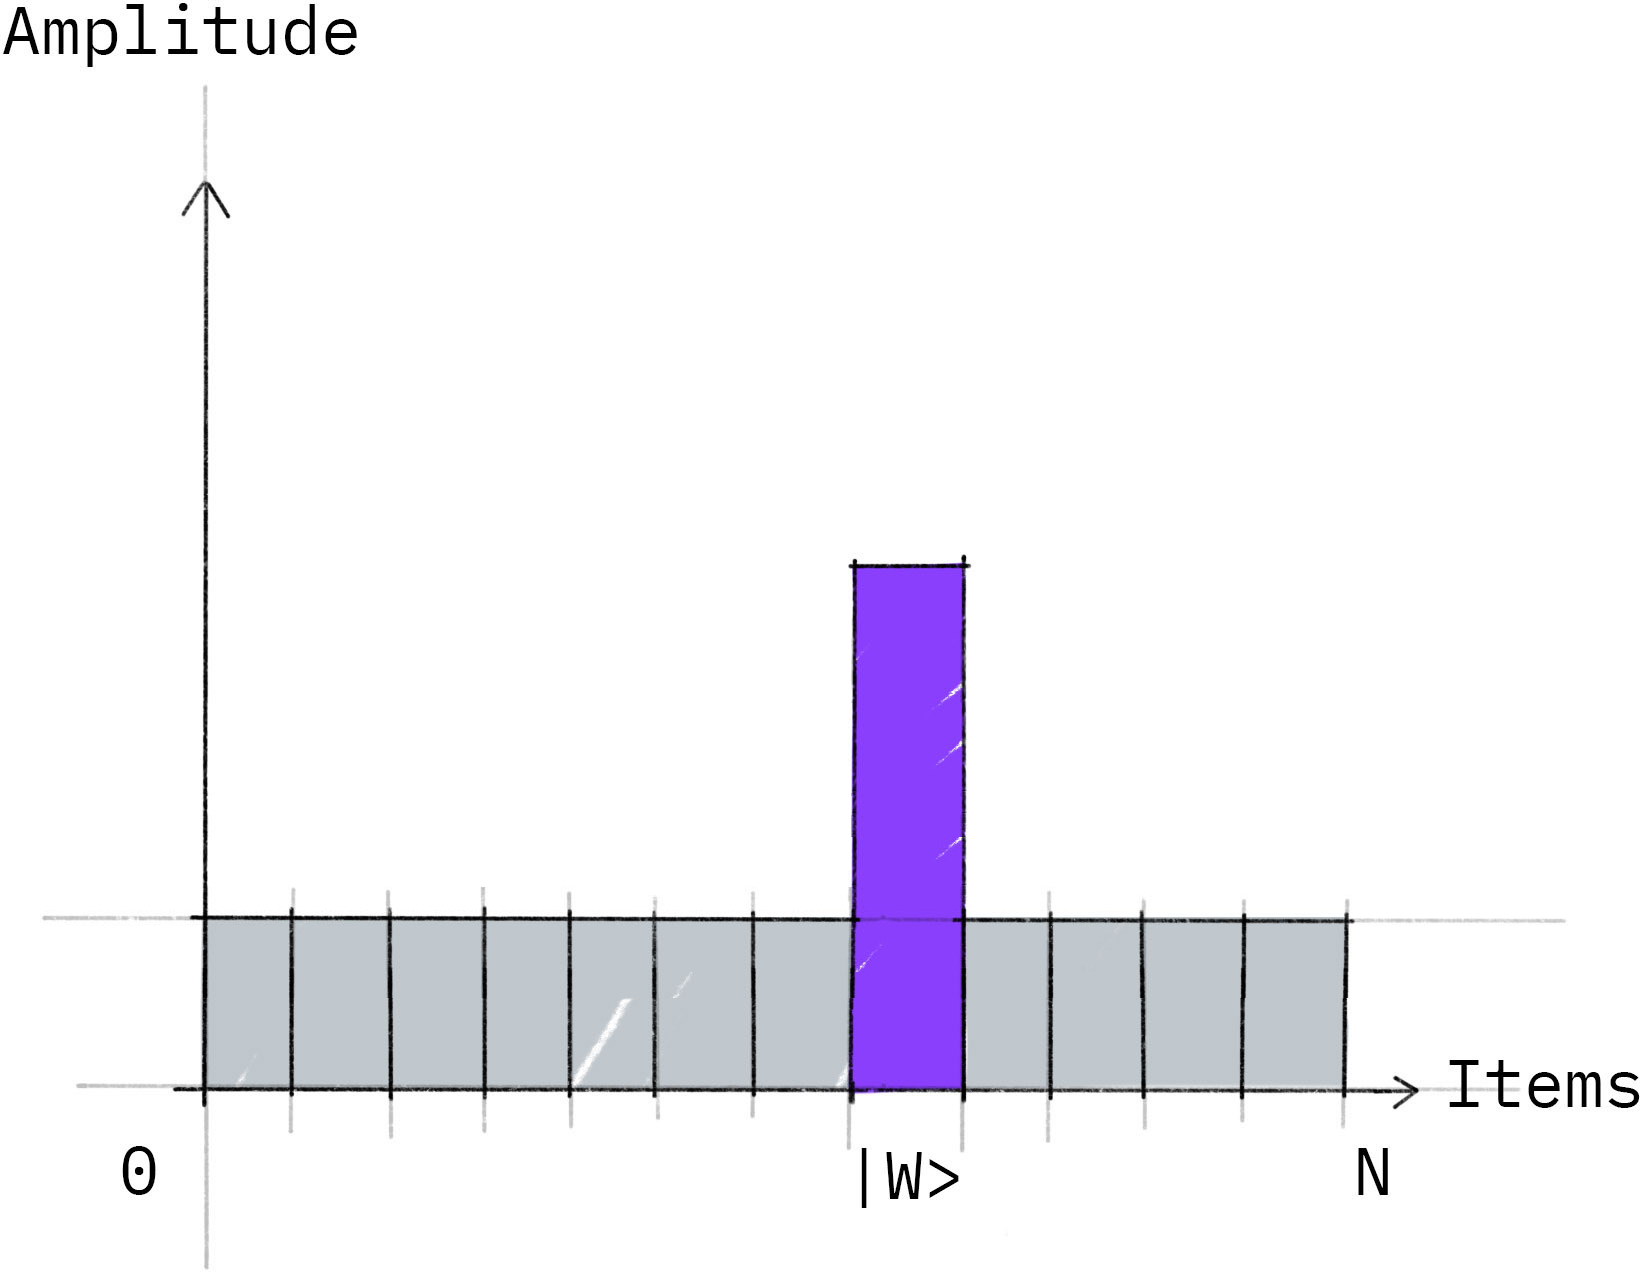
\includegraphics[width=0.5\linewidth]{content/assets/03_grovers_algorithm/grover_final.jpg}
    \caption{Grover amplifies the amplitude(s) of the correct solution(s)}
    \label{fig:grover_uniform}
\end{figure}

Finally, it samples from this probability distribution, which results in a correct solution entity with a high chance.

Working with a probability distribution over an exponentially large set of entities is only possible in a memory-efficient way on a quantum computer, thanks to the quantum physical nature of qubits.

A register of classical bits can only represent a single entity (encoded as a binary number), we would need separate registers to represent a set and we can only operate on the entire set in a linear fashion, one register at a time. In contrast, a register of quantum bits, or 'qubits' itself can represent a set of entities (a set of binary numbers) from the domain using the quantum physical phenomenon of superposition with a probability distribution over these elements.

The manipulation of these probabilities happens using quantum operators or gates, which are the basis of all quantum algorithms on gated general-purpose quantum computers.

However, we do not have access to this probability distribution or the high probability elements in it. The only thing we can do is read the register, which is an operation that samples a single entity from the current probability distribution in the register, destroying it in the process. We are unable to 'iterate' the contents of the register or know what the probability of the resulting element was from the sampling.

This is the reason why quantum parallelism is not as trivial as the name suggests: while we can run the computation itself in parallel, gaining access to the information that we stored in the register is difficult and destructive. Amplitude amplification is a technique that we use to fix this problem, however it requires $O(\sqrt{N})$ time, where $N$ is the size of the problem's domain, where $N=2^n$ if the quantum register has $n$ qubits.

One of the most important property of quantum registers is that they can even represent probability distributions, even ones where the individual qubits are \textbf{not independent}. This is called quantum entanglement.

The simplest forms of quantum entanglement are Bell states, which can occur between two qubits. In one of these Bell states, the probability distribution of our 2 qubit quantum registers is "$00$" with $50\%$ probability and "$11$" with $50\%$. Reading the contents of just the first qubit will result in a $50\%$ chance of reading a $0$ and a $50\%$ chance of reading a $1$. However, once we know the result from the first qubit, we can be $100\%$ sure, that when we sample the second qubit, we will get the same number as a result from it.

\section{Showcasing the algorithm on a simple task}

In the original Sudoku puzzle, we have a $(3^2\cdot{}3^2)$ table, that must be filled with numbers between $1$ and $9$. A correct solution to a puzzle is where each row, column and distinct $(3\cdot{}3)$ square has unique numbers.

\begin{figure}[H]
  \centering
  \begin{subfigure}{.49\linewidth}
    \centering
    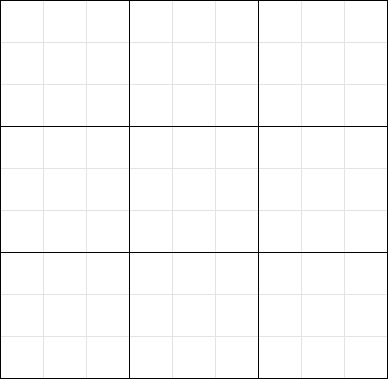
\includegraphics[width=\linewidth]{content/assets/03_grovers_algorithm/sudoku_3_empty.png}
    \caption{Empty}
  \end{subfigure}
  \begin{subfigure}{.49\linewidth}
    \centering
    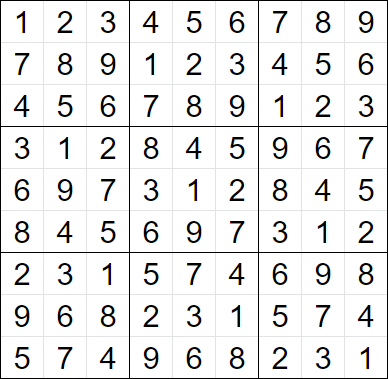
\includegraphics[width=\linewidth]{content/assets/03_grovers_algorithm/sudoku_3_solution.png}
    \caption{Solved}
  \end{subfigure}
  \caption{Sudoku puzzle}
\end{figure}

In order demonstrate memory usage scaling, I generalize this Sudoku to a table of size $(n^2\cdot{} n^2)$, where each row, column and $(n\cdot{}n)$ distinct subsquare of the table must be a unique number from the $[1, n^2]$ interval.

The only solution for $n=1$ is trivial.

\begin{figure}[H]
  \centering
  \begin{subfigure}{.4\linewidth}
  \end{subfigure}
  \begin{subfigure}{.1\linewidth}
    \centering
    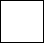
\includegraphics[width=0.6\linewidth]{content/assets/03_grovers_algorithm/sudoku_1_empty.png}
    \caption{Empty}
  \end{subfigure}
  \begin{subfigure}{.1\linewidth}
    \centering
    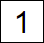
\includegraphics[width=0.6\linewidth]{content/assets/03_grovers_algorithm/sudoku_1_solution.png}
    \caption{Solved}
  \end{subfigure}
  \begin{subfigure}{.4\linewidth}
  \end{subfigure}
  \caption{Sudoku puzzle $(n=1)$}
\end{figure}

An example solution for $n=2$.

\begin{figure}[H]
  \centering
  \begin{subfigure}{.25\linewidth}
  \end{subfigure}
  \begin{subfigure}{.25\linewidth}
    \centering
    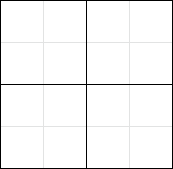
\includegraphics[width=\linewidth]{content/assets/03_grovers_algorithm/sudoku_2_empty.png}
    \caption{Empty}
  \end{subfigure}
  \begin{subfigure}{.25\linewidth}
    \centering
    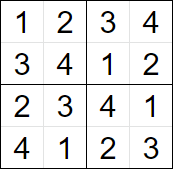
\includegraphics[width=\linewidth]{content/assets/03_grovers_algorithm/sudoku_2_solution.png}
    \caption{Solved}
  \end{subfigure}
  \begin{subfigure}{.25\linewidth}
  \end{subfigure}
  \caption{Sudoku puzzle $(n=2)$}
\end{figure}

$n=3$ is normal Sudoku.

And an example for $n=4$ is the following:

\begin{figure}[H]
  \centering
  \begin{subfigure}{.49\linewidth}
    \centering
    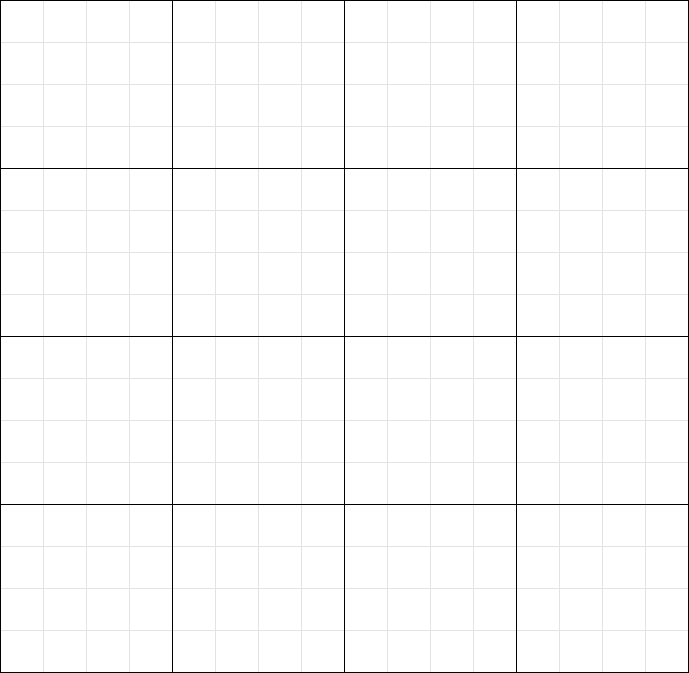
\includegraphics[width=\linewidth]{content/assets/03_grovers_algorithm/sudoku_4_empty.png}
    \caption{Empty}
  \end{subfigure}
  \begin{subfigure}{.49\linewidth}
    \centering
    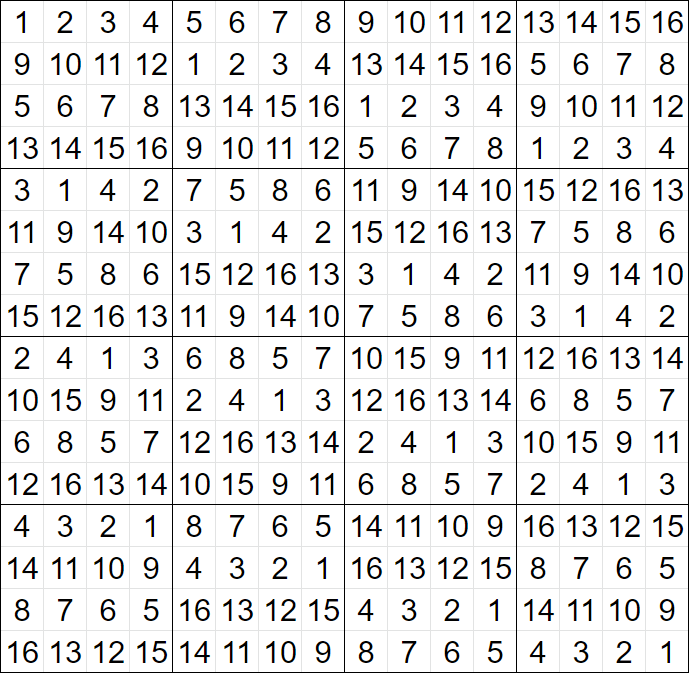
\includegraphics[width=\linewidth]{content/assets/03_grovers_algorithm/sudoku_4_solution.png}
    \caption{Solved}
  \end{subfigure}
  \caption{Sudoku puzzle $(n=4)$}
\end{figure}

\section{Designing a quantum solver for the Sudoku puzzle}

In this section I first define the Sudoku problem's representation in a binary form, then design the verifier algorithm (quantum oracle) for the puzzle, finally I go over the remaining parts of Grover's framework and the amplitude amplification technique it uses.

\subsection{Register definitions}

The first step is to encode the problem using quantum registers. The size-$n$ Sudoku table has $n^2$ rows and columns. Every cell in it is represented by a quantum register:

\begin{align*}
\text{cell}[i][j] = \ket{0\dots{}010\dots{}0}, & \hspace{3mm}\forall{}\hspace{1mm}(0\leq{}i,j<n^2).
\end{align*}

The length (qubits) of the register is $n^2$ and the number in the cell is represented using one-hot encoding. One-hot encoding means, that a number between $0$ and $b-1$ is represented by a $b$ bit register, each number corresponding to a single bit being $1$ in the register:

\begin{align*}
\text{cell}[i][j][k] = \begin{cases}
\ket{1} & \text{cell}_{(i,j)}\text{'s number is }(k+1) \\
\ket{0} & \text{otherwise}
\end{cases}, & \hspace{3mm}\forall{}(\hspace{1mm}0\leq{}i,j,k<n^2).
\end{align*}

In Qiskit, once the qubit registers are added to a circuit, they can be indexed using a single dimensional index, such as:

\begin{align*}
\text{cell}[i][j][k] = \text{cell}[i\cdot{}n^4+j\cdot{}n^2+k], & \hspace{3mm}\forall{}\hspace{1mm}(0\leq{}i,j,k<n^2).
\end{align*}

\subsection{Oracle operator}

\subsubsection{Constraint definitions}

I will verify if a solution is correct, using uniqueness constraints. These constraints will all be using the same scheme, which I define as UNIQUE\_ONE($[x_0,\dots,{}x_{n-1}]$) constraint, where $[x_0,\dots,{}x_{n-1}]$ is a list of single-dimensional indexes. If a UNIQUE\_ONE($[x_0,\dots,{}x_{n-1}]$) constraint is applied, the qubits with indexes $[x_0,\dots,{}x_{n-1}]$ must contain exactly one $\ket{1}$.

The verifications are the following:

\textbf{Cells should be one-hot encoded}

Every $(i,j)$ row and column index pair corresponds to a cell. The qubits in this cells, indexed by $k$ shall have a single $\ket{1}$ among them.

\begin{align*}
    \text{UNIQUE\_ONE}([i\cdot{}n^4 + j\cdot{}n^2 + k]_{0\leq{}k<n^2}), & \hspace{3mm} \forall{}0\leq{}i,j<n^2
\end{align*}

\textbf{Numbers in each row should be unique}

For every $i$ row and every $k$ one-hot encoded number position, the $k$ number should be present in the $i$th row exactly once, indexed by the $j$ columns:

\begin{align*}
    \text{UNIQUE\_ONE}([i\cdot{}n^4 + j\cdot{}n^2 + k]_{0\leq{}j<n^2}), & \hspace{3mm} \forall{}0\leq{}i,k<n^2
\end{align*}

\textbf{Numbers in each column should be unique}

For every $j$ column and every $k$ one-hot encoded number position, the $k$ number should be present in the $j$th column exactly once, indexed by the $i$ rows:

\begin{align*}
    \text{UNIQUE\_ONE}([i\cdot{}n^4 + j\cdot{}n^2 + k]_{0\leq{}i<n^2}), & \hspace{3mm} \forall{}0\leq{}j,k<n^2
\end{align*}

\textbf{Numbers in each square should be unique}

In order to create this constraint, the row and column indexes must be taken apart into an inner and outer index:

\begin{align*}
i = i_{outer}\cdot{}n + i_{inner},\hspace{3mm}& (0\leq{}i_{outer},i_{inner}<n) \\
j = j_{outer}\cdot{}n + j_{inner},\hspace{3mm}& (0\leq{}j_{outer},j_{inner}<n) \\
\end{align*}

This way $i_{outer}$ and $j_{outer}$ index the squares the constraint is applied to, while $i_{inner}$ and $j_{inner}$ index their internal cells.

Then, for every square, indexed by the $(i_{outer}, j_{outer})$ pair and every $k$ one-hot encoded number position, the $k$ number should be present in the $(i_{outer}, j_{outer})$ square exactly once, indexed by the $(i_{inner}, j_{inner})$ cell index pairs:

\begin{align*}
    \text{UNIQUE\_ONE}([(i_{outer}\cdot{}n + i_{inner})\cdot{}n^4 + (j_{outer}\cdot{}n + j_{inner})\cdot{}n^2 + k]_{0\leq{}i_{inner},j_{inner}<n}), \\ \forall{}0\leq{}i_{outer},j_{outer}<n,\forall{}0\leq{}k<n^2
\end{align*}

\subsubsection{Implementation of the UNIQUE\_ONE constraint}

In order to implement a UNIQUE\_ONE($[x_0,\dots,{}x_{n-1}]$) constraint, we use the WeightedAdder component from Qiskit. This takes $n$ qubits and sums them up into a $\log_{2}(n)$ sized array. We want the sum to be exactly $1$, which means that the output of the sum array should be equal to $\ket{0\dots{}01}$. Adding a $NOT$ gate to the least significant qubit, the output should be $\ket{0\dots{}0}$. This can be tested using a multi-controlled $NOT$, or $M-CNOT$ gate.

\begin{figure}[H]
  \centering
    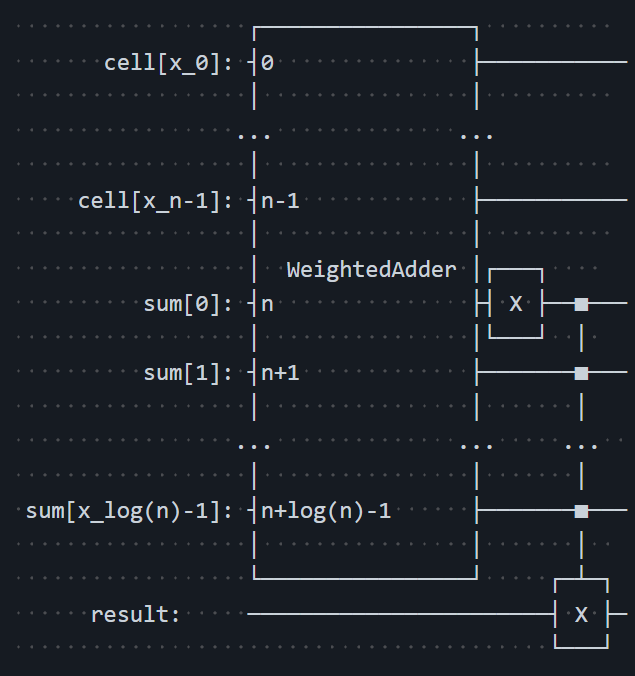
\includegraphics[width=0.7\linewidth]{content/assets/03_grovers_algorithm/unique_one.png}
    \caption{Unique one (TODO fehér diagram)}
\end{figure}

For multiple UNIQUE\_ONE constraints, the results can be aggregated using a final multi-controlled $CNOT$ gate, or using a single, common $M-CNOT$ gate for all of them.

In the end, this final $MCNOT$ operation is applied to a single, $\ket{oracle}$ qubit in the circuit.

\subsection{Grover's framework: The amplitude amplification technique}

This chapter is based on the chapter on Grover's algorithm from the Qiskit Texbook\cite{GroverQiskitTextbook}.

Let us denote the $cells[i][j][k]$ qubits with the $\ket{cells}$ qubit vector!

In the beginning, Grover initializes this vector to the uniform distribution:

\begin{align*}
\ket{s} = \frac{1}{\sqrt{N}}\sum\limits_{x=0}^{N-1}\ket{x}
\end{align*}

This is done by applying an $n$-dimensional Hadamard-matrix to the $\ket{0\dots{}0}$ vector.

\begin{align*}
\ket{s} = H^{\otimes{}n}\ket{0}
\end{align*}

We can see this initial state in the following figure.

\begin{figure}[H]
  \centering
    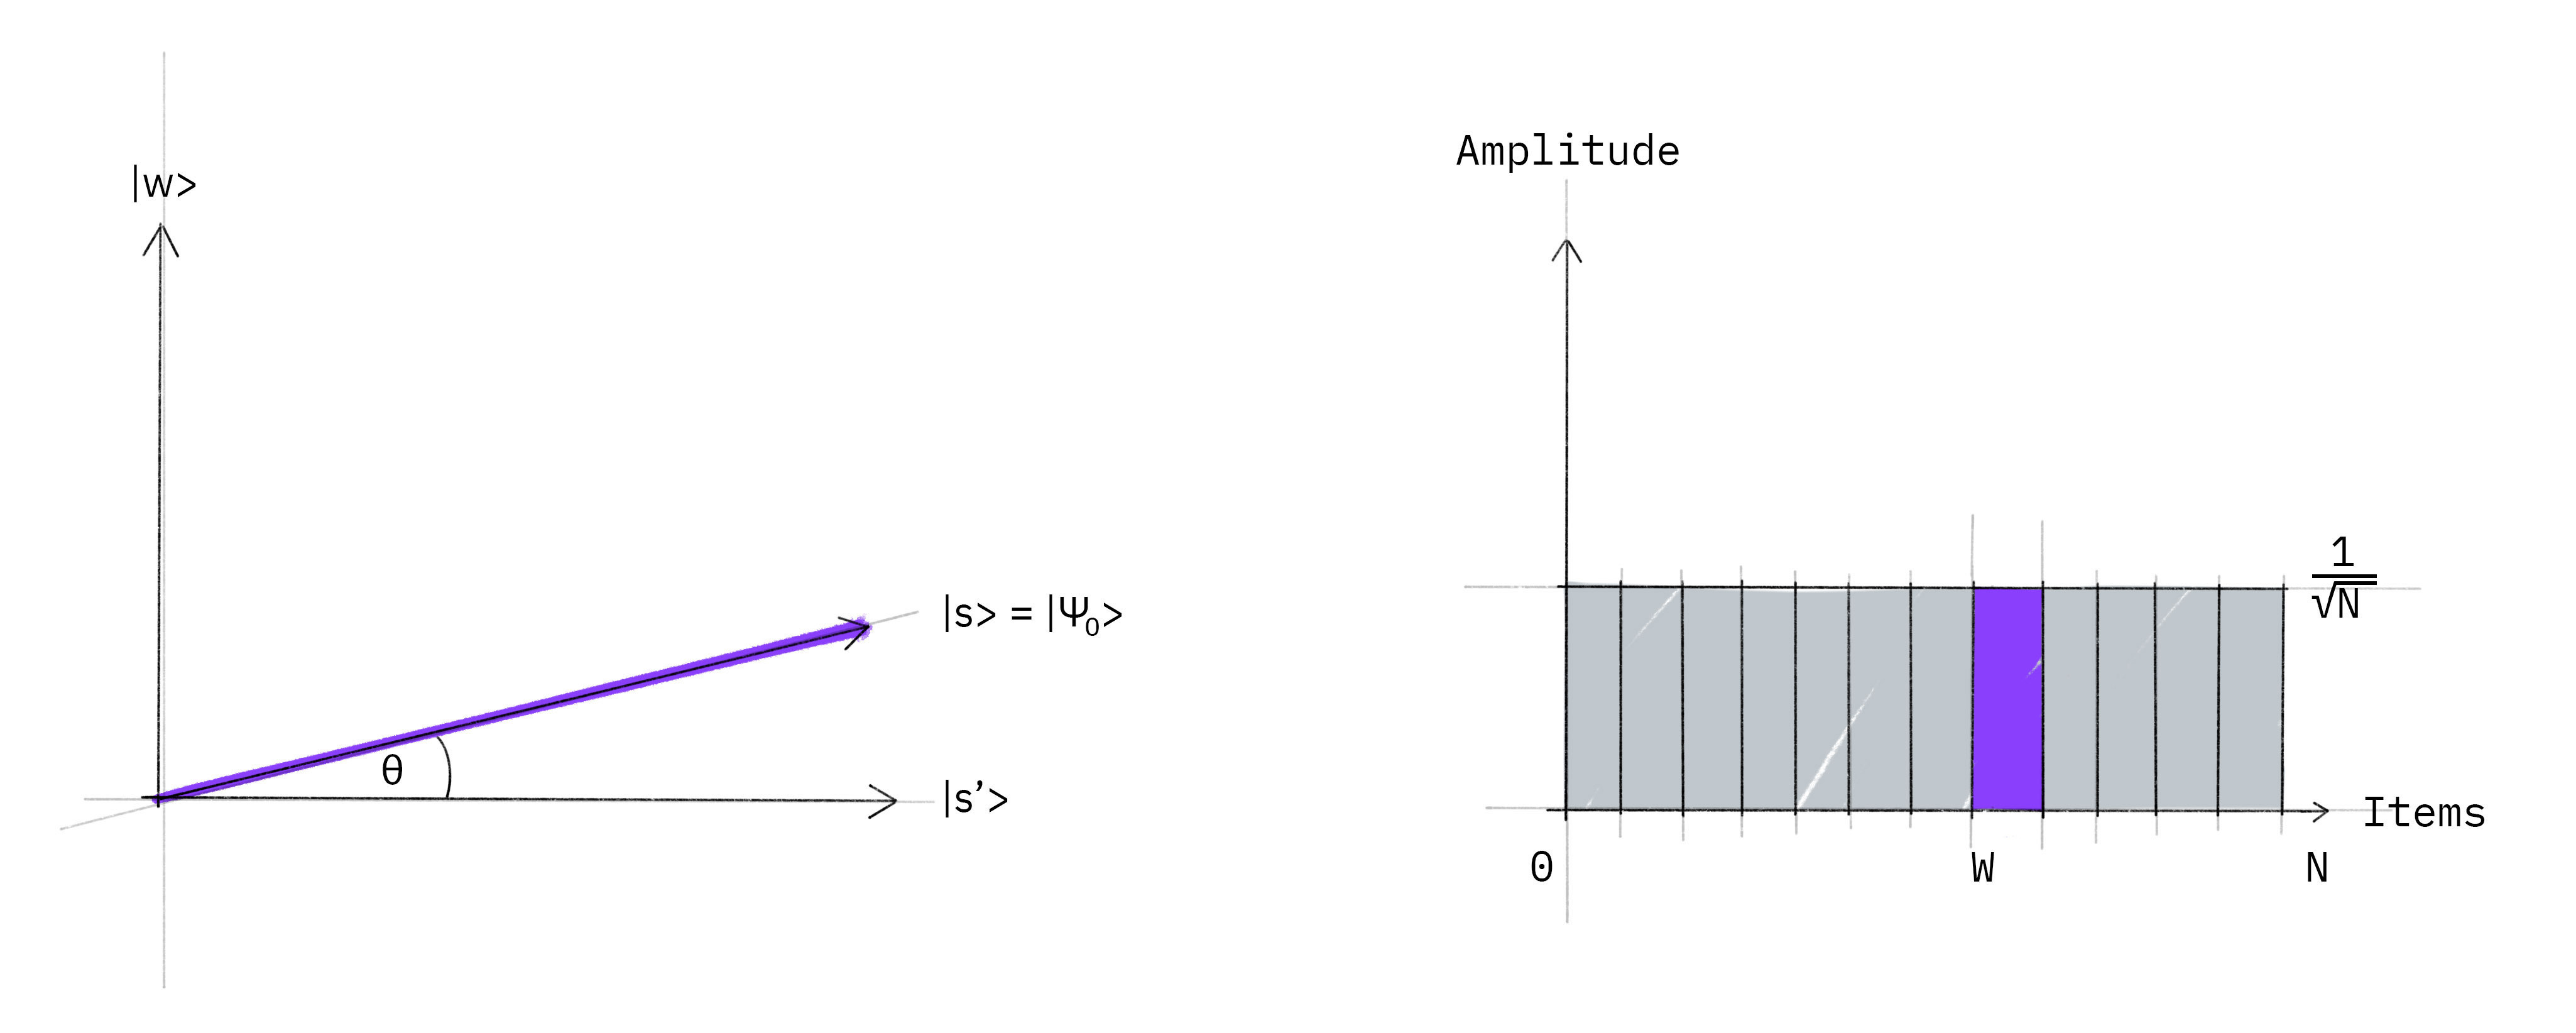
\includegraphics[width=\linewidth]{content/assets/03_grovers_algorithm/grover_step1.jpg}
    \caption{Initialization}
\end{figure}

On the right hand side, the individual amplitudes are represented for all elements in the $\ket{cells}$ vector. This can be seen as an $N$-dimensional vector. Since we are only interested in what is the probability of sampling a correct solution, we can project this $N$-dimensional vector-space into a $2$-dimensional one, where the dimensions correspond to the probability of a solution and a non-solution sampling. The $x$-axis, or $\ket{s'}$ represents non-solutions, while the $y$-axis, or $\ket{w}$ represents the solutions.

In order to create a Grover's oracle from the oracle function defined in the previous section, I initialize the $\ket{oracle}$ qubit to $\ket{-} = \frac{1}{\sqrt{2}}\ket{0} - \frac{1}{\sqrt{2}}\ket{1}$. When the oracle circuit is applied to $\ket{oracle} = \ket{-}$, the phase kickback effect results in a negative amplitude multiplier exactly on the elements in the $\ket{cells}$ vector, which are solutions according to the oracle.

This effect can be seen on these figures:

\begin{figure}[H]
  \centering
    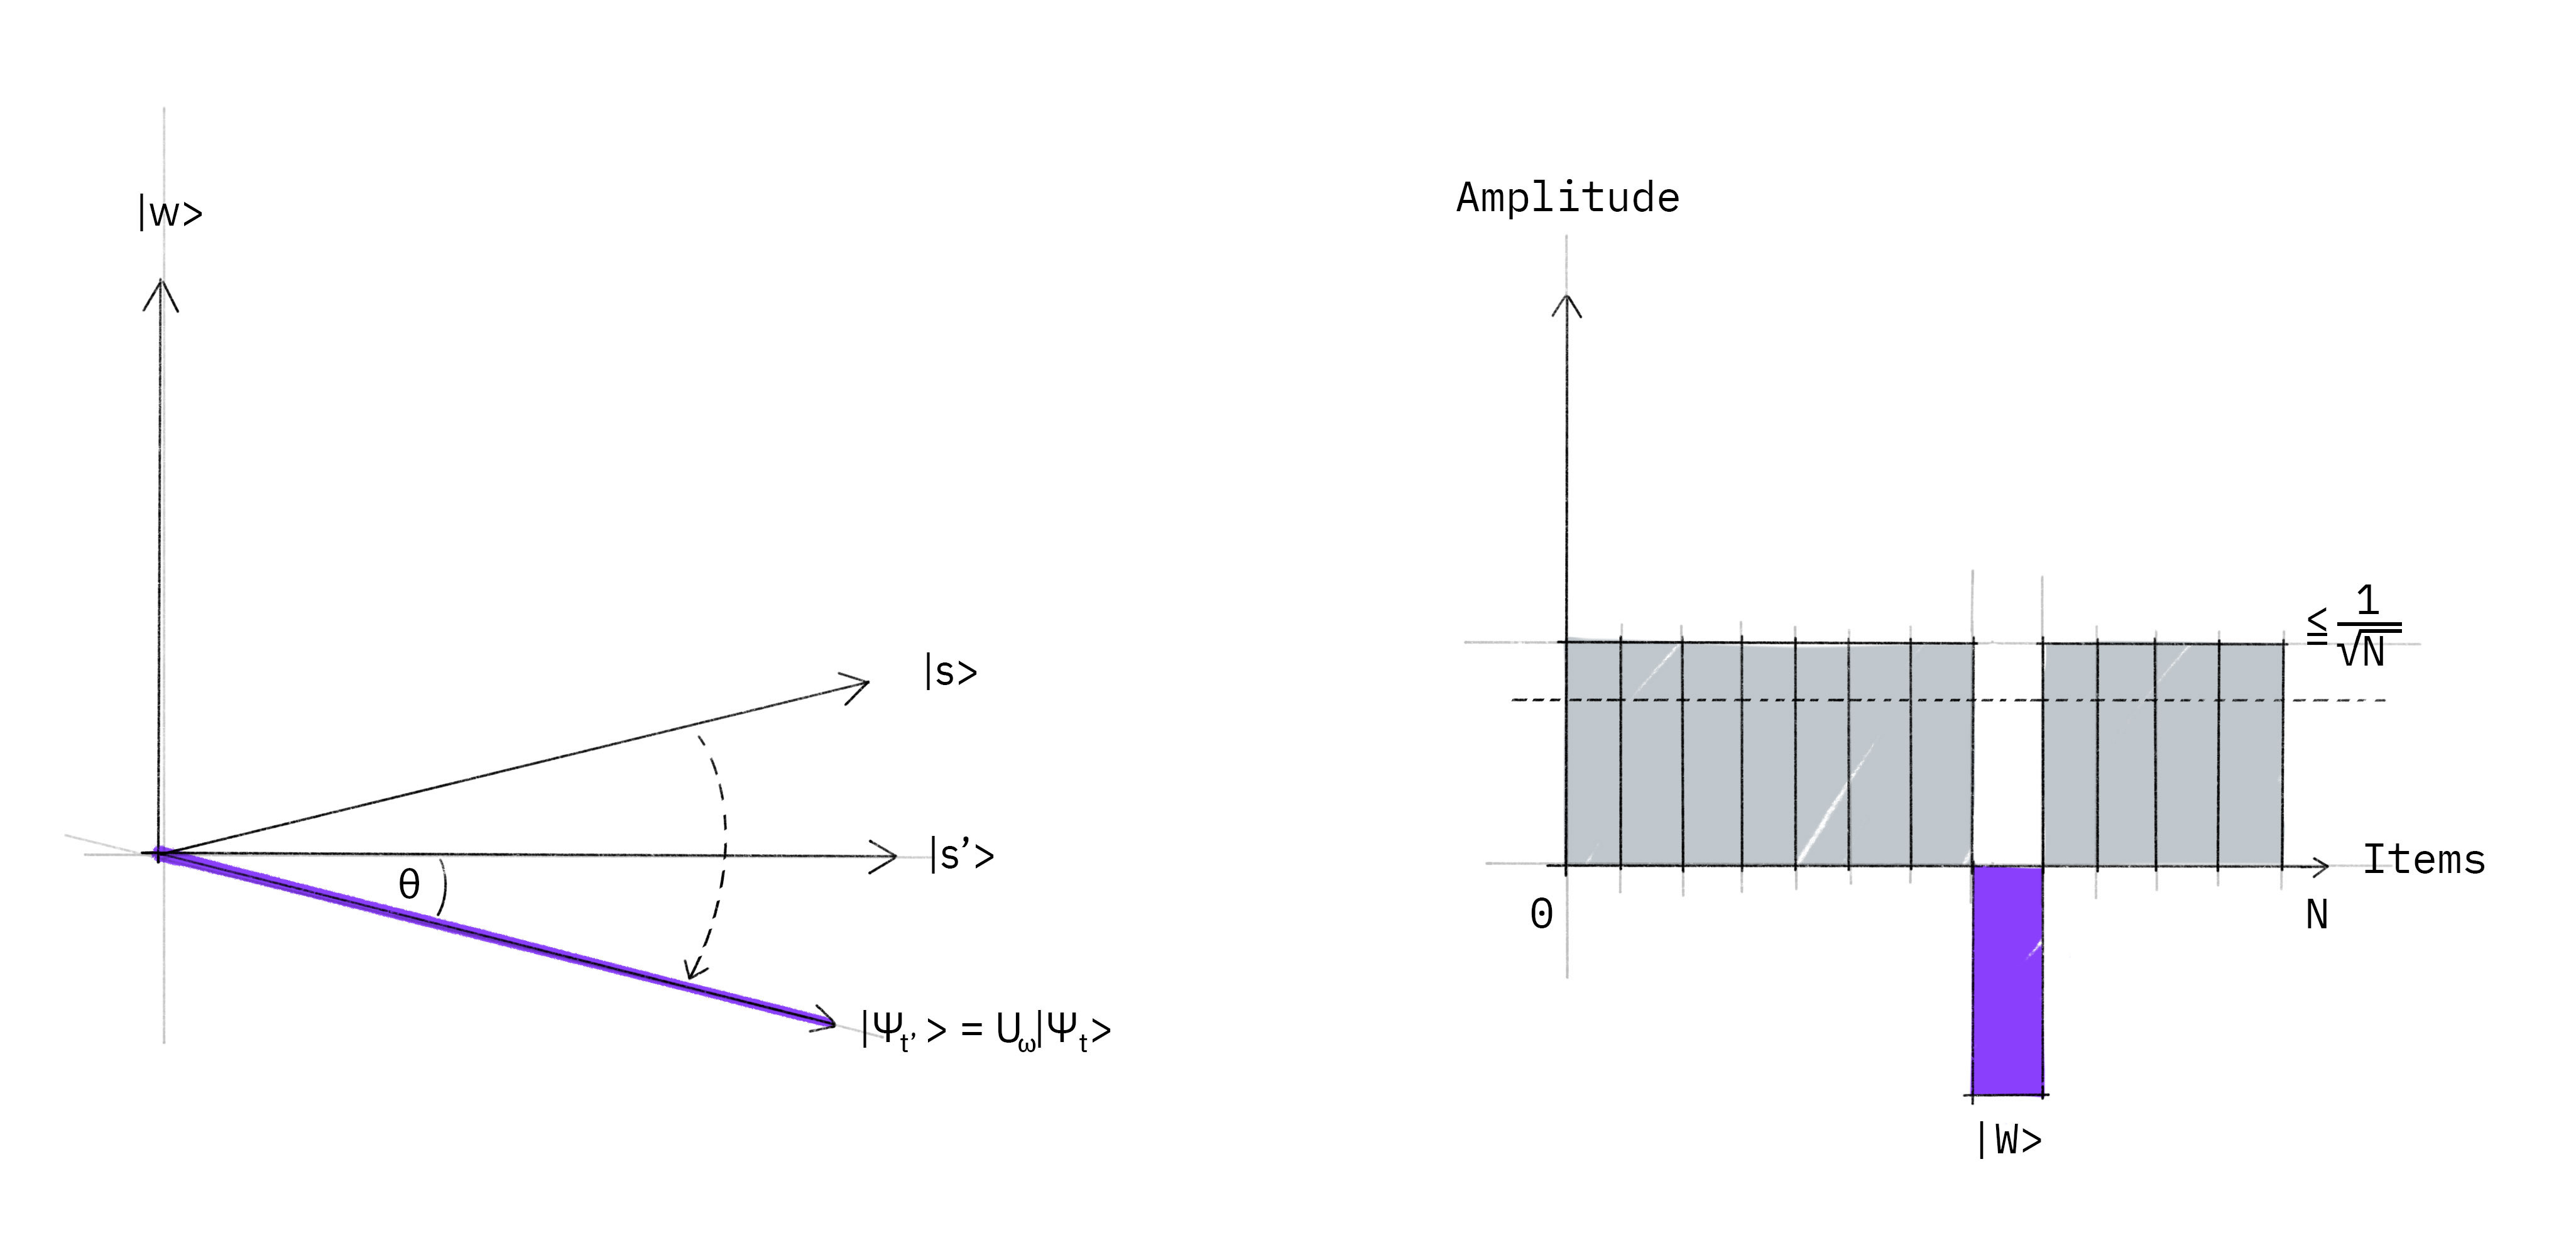
\includegraphics[width=\linewidth]{content/assets/03_grovers_algorithm/grover_step2.jpg}
    \caption{Phase kickback}
\end{figure}

On the right-hand side, the solutions amplitudes are flipped. Since the solutions constutire the $y$-axis on the left-hand side, this results in a reflection over the $x$-axis.

Finally, another reflection is performed, which reflexts over the average amplitude in the current superposition. For non-solution elements this decreases their overall probability, while the flipped solution elements gain probability.
\begin{figure}[H]
  \centering
    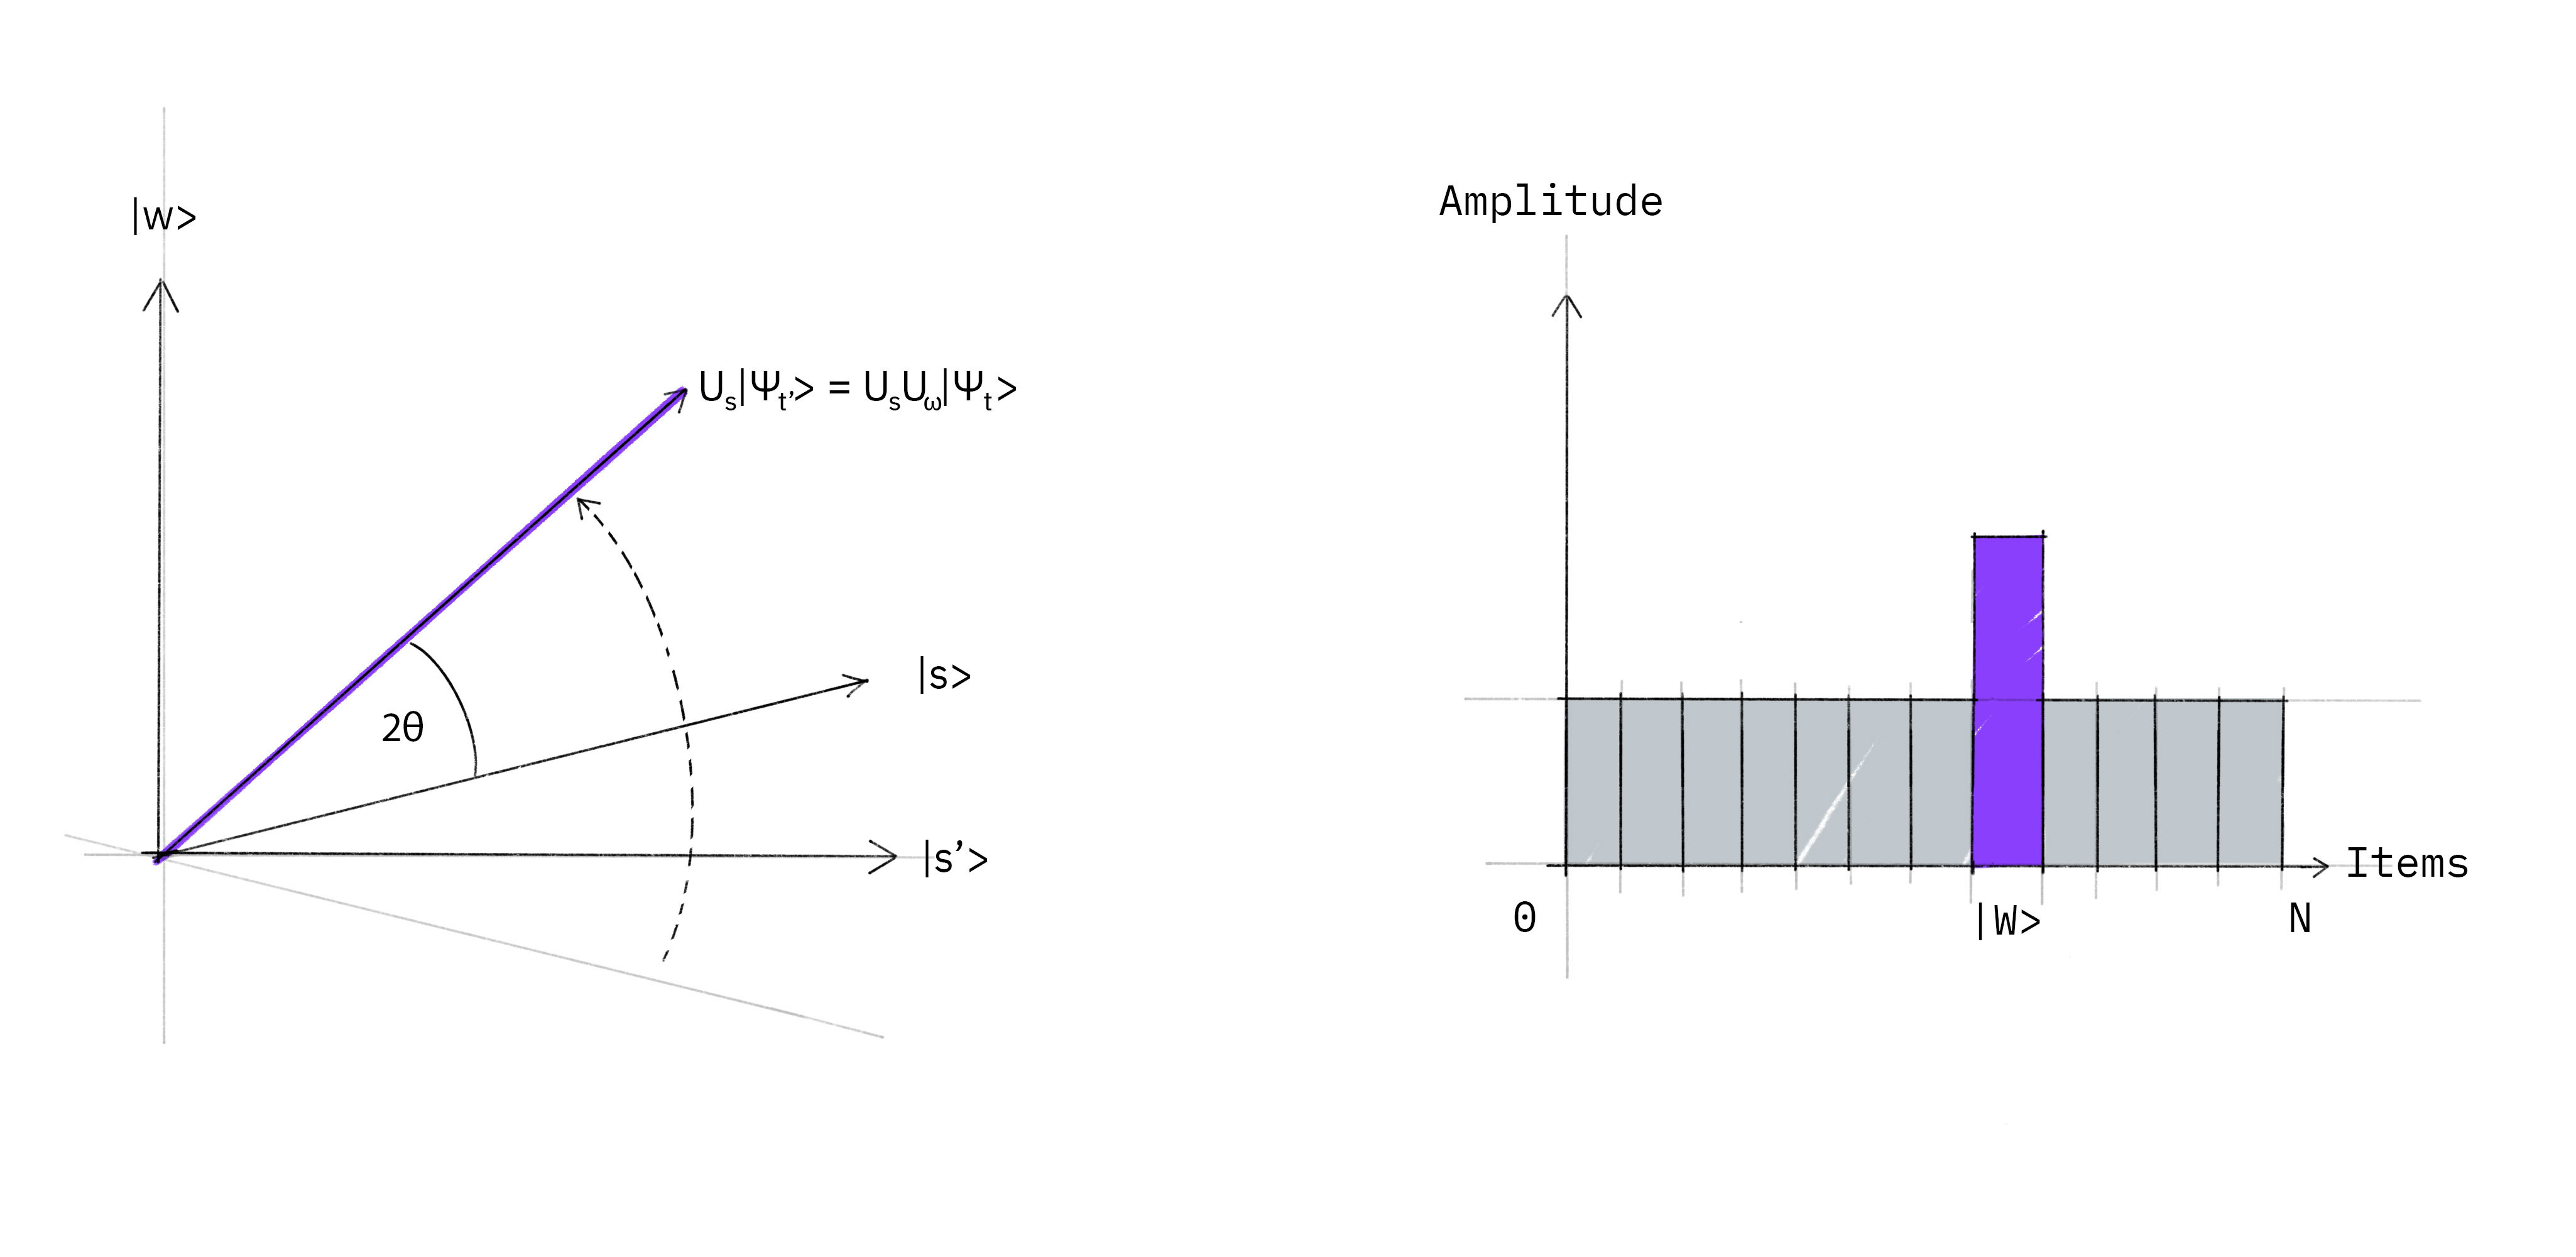
\includegraphics[width=\linewidth]{content/assets/03_grovers_algorithm/grover_step3.jpg}
    \caption{Reflect over the average amplitude}
\end{figure}

On the left-hand side this can be represented by a reflextion over the initial (uniform) distribution, the $\ket{s}$ vector. This operation is called the diffuser operator, which is implemented by a Grover matrix.

Together, these two reflections constitute a rotation towards the $\ket{w}$ solution axis with a degree that depends on the size of the search space ($N$) and the number of solutions ($M$). In order to reach the $\ket{w}$ axis as close as possible, the rotation must be performed $\sqrt{\frac{N}{M}}$ times.

In order to recompute the oracle on the new search space, first the old results must be erased from the ancilla (sum) qubits in the system. Since the WeightedAdder operator works internally with $CNOT$ gates, erasing the result can be done by applying the same circuit in reverse order.

\section{The tools needed to implement Grover's algorithm}

In this capter I have introduced Grover's algorithm and how to use it to solve a generalized version of the Sudoku puzzle.

In order to use this framework, 4 operators must be implemented in the system: the Hadamard (for the phase-kickback), the Grover (the diffuser operator), the Sum (WeightedAdder) and the Multi-controlled NOT gate (for the oracle bit).
